\documentclass[times]{itmo-student-thesis}

%% Опции пакета:
%% - specification - если есть, генерируется задание, иначе не генерируется
%% - annotation - если есть, генерируется аннотация, иначе не генерируется
%% - times - делает все шрифтом Times New Roman, собирается с помощью xelatex
%% - languages={...} - устанавливает перечень используемых языков. По умолчанию это {english,russian}.
%%                     Последний из языков определяет текст основного документа.

%% Делает запятую в формулах более интеллектуальной, например:
%% $1,5x$ будет читаться как полтора икса, а не один запятая пять иксов.
%% Однако если написать $1, 5x$, то все будет как прежде.
\usepackage{icomma}

%% Один из пакетов, позволяющий делать таблицы на всю ширину текста.
\usepackage{booktabs}   % красивые линии
\usepackage{tabularx}   % таблицы на всю ширину
\usepackage{array}      % доп. выравнивание
\usepackage{makecell}   % перенос строк в ячейках
%% Данные пакеты необязательны к использованию в бакалаврских/магистерских
%% Они нужны для иллюстративных целей
%% Начало
\usepackage{tikz}
\usetikzlibrary{arrows}
\usepackage{filecontents}
\usepackage{graphicx}
\usepackage{float}
%% Конец

%% Указываем файл с библиографией.
\addbibresource{bachelor-thesis.bib}

\begin{document}

\studygroup{M3437}
\title{Разработка программного модуля поддержки YDB в системе Keycloak в качестве основного хранилища данных}
\author{Мухтаров Айнур Дамирович}{Мухтаров А.Д.}
\supervisor{Аксенов Виталий Евгеньевич}{Аксенов В.Е.}{д.т.н.}{главный научный сотрудник Университета ИТМО}
\publishyear{2026}
%% Дата выдачи задания. Можно не указывать, тогда надо будет заполнить от руки.
\startdate{}{}{}
%% Срок сдачи студентом работы. Можно не указывать, тогда надо будет заполнить от руки.
\startdate{}{}{}
%% Дата защиты. Можно не указывать, тогда надо будет заполнить от руки.
\defencedate{}{}{}

% \begin{filecontents}{bachelor-thesis.bib}{

% % ------------------------------------------------------------------
% % 1. YDB / YANDEX DATABASE
% % ------------------------------------------------------------------

% @online{ydb_github,
%   author       = {{YDB Platform}},
%   title        = {{YDB: Open Source Distributed SQL Database}},
%   howpublished = {GitHub Repository / Official Website},
%   year         = {2022},
%   url          = {https://www.keycloak.org/},
%   langid       = {english}
% }

% @online{ydb_liquibase_driver,
%   author       = {{YDB Platform}},
%   title        = {{YDB Liquibase dialect}},
%   howpublished = {GitHub Repository},
%   url          = {https://github.com/ydb-platform/ydb-java-dialects},
%   langid       = {english}
% }

% @online{ydb_liquibase_driver,
%   author       = {{YDB Platform}},
%   title        = {{YDB Hibernate dialect}},
%   howpublished = {GitHub Repository},
%   url          = {https://github.com/ydb-platform/ydb-java-dialects},
%   langid       = {english}
% }

% % ------------------------------------------------------------------
% % 2. KEYCLOAK
% % ------------------------------------------------------------------

% @online{keycloak,
%   author       = {{Keycloak}},
%   year         = {2014},
%   howpublished = {GitHub Repository / Official Website},
%   title        = {Keycloak - Open Source Identity and Access Management},
%   url          = {https://github.com/keycloak/keycloak},
%   langid       = {english}
% }

% % ------------------------------------------------------------------
% % 3. ORM / JAVA PERSISTENCE
% % ------------------------------------------------------------------
% % hibernate
% @online{jsr338,
%   author       = {{Hibernate}},
%   title        = {{Hibernate ORM framework}},
%   howpublished = {GitHub Repository / Official Website},
%   year         = {2001},
%   url          = {https://hibernate.org/},
%   langid       = {english}
% }

% % ------------------------------------------------------------------
% % 4. DATABASE MIGRATION TOOLING
% % ------------------------------------------------------------------

% @online{liquibase_github,
%   author       = {{Liquibase}},
%   title        = {{Liquibase: Database Schema Change Management}},
%   howpublished = {GitHub Repository / Official Website},
%   year         = {2023},
%   url          = {https://www.liquibase.org},
%   langid       = {english}
% }

% % ------------------------------------------------------------------
% % 9. LOAD TESTING
% % ------------------------------------------------------------------

% @online{keycloak_benchmark,
%   author       = {{Keycloak}},
%   title        = {{Keycloak benchmark}},
%   howpublished = {GitHub Repository / Official Website},
%   url          = {https://www.keycloak.org/keycloak-benchmark/},
%   note         = {Tools to run performance tests of a Keycloak server.},
%   langid       = {english}
% }

% @online{gatling_github,
%   author       = {{Gatling Corp}},
%   title        = {{Gatling: Modern Load Testing as Code}},
%   howpublished = {GitHub Repository},
%   year         = {2012},
%   url          = {https://github.com/gatling/gatling},
%   note         = {Open-source load-testing framework built on Scala, Akka,
%                   and Netty; single agent sustains 3\,000--5\,000+ virtual
%                   users.},
%   langid       = {english}
% }

% }
% TODO
% МБ Кирилла Сюда хз
% \addconsultant{Белашенков Н.Р.}{канд. физ.-мат. наук, без звания}
% \addconsultant{Беззубик В.В.}{без степени, без звания}

\secretary{Штумпф С. А.}

%% Эта команда генерирует титульный лист и аннотацию.
\maketitle{Бакалавр}

%% Оглавление
\tableofcontents

%% Макрос для введения. Совместим со старым стилевиком.
\startprefacepage

В современных распределённых системах управление идентификацией и доступом
(Identity and Access Management, IAM) является важным компонентом
инфраструктуры. Keycloak --- IAM-система с открытым исходным кодом, разработанная
компанией Red Hat, --- предоставляет единый вход (SSO), поддержку протоколов
OAuth 2.0, OpenID Connect и SAML, управление пользователями и двухфакторную
аутентификацию. Keycloak широко применяется в современных приложениях
как готовое решение для обеспечения безопасности приложений.

Keycloak поддерживает только реляционные СУБД: PostgreSQL, MySQL, MariaDB,
Oracle, TiDB и Microsoft SQL Server. По мере роста нагрузки на систему 
узким местом становится хранилище данных. Традиционные РСУБД масштабируются
преимущественно вертикально и требуют значительных усилий для обеспечения
отказоустойчивости в распределённых сценариях.

YDB (Yandex Database) --- распределённая NewSQL-СУБД с открытым исходным кодом,
разработанная Яндексом. В отличие от большинства распределённых СУБД, жертвующих 
согласованностью ради масштабируемости, YDB обеспечивает горизонтальное масштабирование
и высокую доступность \textit{одновременно} с полноценными ACID-транзакциями уровня
изоляции \textit{Serializable}. Это делает YDB привлекательной альтернативой для
организаций, которым требуется легко масштабируемое хранилище без отказа от
транзакционных гарантий.

Вместе с тем официальной поддержки YDB в Keycloak не существует: отсутствует
совместимый Hibernate-диалект для актуальной версии фреймворка, а ряд
конструкций, генерируемых Keycloak, несовместим с диалектом YQL.

Целью работы является разработка программного модуля, обеспечивающего интеграцию
Keycloak с YDB в качестве основного хранилища данных.

Практическая значимость работы состоит в том, что разработанный модуль позволяет
организациям, уже использующим YDB в своей инфраструктуре, развернуть Keycloak
без необходимости поддерживать отдельную реляционную СУБД.

Новизна работы заключается в разработке открытого решения, обеспечивающего
интеграцию Keycloak с YDB через механизм SPI.

Работа состоит из четырёх глав. В главе~1 проведён анализ предметной области:
рассмотрена архитектура Keycloak и механизм SPI, описана СУБД YDB и её свойства,
выполнен обзор существующих решений по интеграции Keycloak с нереляционными
хранилищами. В главе~2 описано проектирование решения: общая архитектура модуля,
подход к разработке Hibernate-диалекта и механизм повторного выполнения транзакций.
В главе~3 представлена реализация: диалект Hibernate v7, SPI-провайдеры и механизм
переопределения именованных запросов. В главе~4 описано тестирование: интеграционные
тесты на тестовом контейнере YDB и нагрузочное тестирование с помощью keycloak-benchmark.

%% Начало содержательной части.
\chapter{Анализ предметной области}

\section{Система управления идентификацией Keycloak}

С технической точки зрения Keycloak представляет собой сервер, которому приложения делегируют
задачи аутентификации, авторизации и управления пользователями, благодаря чему приложения не 
хранят учётные данные пользователей и не реализуют собственную логику.
Так, при аутентификации по протоколу OpenID Connect приложение перенаправляет
пользователя на Keycloak, после успешного входа получает \textit{access token}
и использует его для авторизации последующих запросов без повторного обращения к серверу.

\subsection{Архитектура Keycloak}

Keycloak реализован на основе Quarkus --- Java-фреймворка для создания облачно-ориентированных приложений. 
Для взаимодействия с базой данных используется ORM-фреймворк Hibernate. Управление схемой базы данных
осуществляется через Liquibase.

Центральным элементом расширяемости Keycloak является механизм \texttt{Service Provider Interface (SPI)}.
SPI позволяет заменять внутренние реализации компонентов пользовательскими, сохраняя совместимость с остальными частями системы.

\subsection{Регистрация SPI}

Для подключения собственной реализации через механизм SPI необходимо выполнить следующие шаги.

\textbf{Шаг 1.} Создать класс SPI, реализующий интерфейс \texttt{org.keycloak.provider.Spi}.
Класс описывает точку расширения --- его имя, тип провайдера и тип фабрики.

Например, SPI для подключения к базе данных через JPA выглядит следующим образом:

\begin{lstlisting}
public class JpaConnectionSpi implements Spi {

    @Override
    public boolean isInternal() {
        return true;
    }

    @Override
    public String getName() {
        return "connectionsJpa";
    }

    @Override
    public Class<? extends Provider> getProviderClass() {
        return JpaConnectionProvider.class;
    }

    @Override
    public Class<? extends ProviderFactory> getProviderFactoryClass() {
        return JpaConnectionProviderFactory.class;
    }
}
\end{lstlisting}

\textbf{Шаг 2.} Зарегистрировать SPI и его реализацию через стандартный механизм Java \texttt{ServiceLoader}.
В ресурсы приложения создаются файлы в директории \texttt{META-INF/services/}, содержащие полные имена классов реализаций:

\begin{lstlisting}[
    language={},
    frame=single,
    title={\footnotesize\texttt{META-INF/services/org.keycloak.provider.Spi}},
    backgroundcolor=\color{gray!10}
]
org.keycloak.connections.jpa.JpaConnectionSpi
\end{lstlisting}

\textbf{Шаг 3.} Реализовать интерфейс \texttt{ProviderFactory}.
Фабрика управляет жизненным циклом провайдера и обязана реализовать следующие методы:

\begin{lstlisting}
public interface ProviderFactory<T extends Provider> {
    T create(KeycloakSession session);
    void init(Config.Scope config);
    void postInit(KeycloakSessionFactory factory);
    void close();
    String getId();
    default int order() { return 0; }
}
\end{lstlisting}

\begin{enumerate}
    \item \texttt{create} --- создаёт экземпляр провайдера для каждой сессии;
    \item \texttt{init} --- вызывается один раз при старте сервера;
    \item \texttt{postInit} --- вызывается после инициализации всех фабрик;
    \item \texttt{close} --- вызывается при остановке сервера;
    \item \texttt{getId} --- возвращает уникальный идентификатор реализации;
    \item \texttt{order} --- приоритет среди фабрик (по умолчанию 0).
\end{enumerate}

\textbf{Шаг 4.} Реализовать интерфейс \texttt{Provider}.

Интерфейс \texttt{Provider} --- базовый интерфейс любого провайдера в Keycloak.

\begin{lstlisting}
public interface Provider {
    void close();
}
\end{lstlisting}

Метод \texttt{close()} вызывается по завершении \texttt{KeycloakSession} --- то есть по окончании каждого
HTTP-запроса или транзакции. В нём необходимо освобождать ресурсы, удерживаемые провайдером:
закрывать соединения с базой данных, сбрасывать кэши, завершать транзакции.

Таким образом, жизненный цикл провайдера привязан к сессии: фабрика создаёт новый экземпляр
через \texttt{ProviderFactory.create(session)} в начале каждой сессии, а Keycloak вызывает
\texttt{close()} при её завершении.

\begin{figure}[H]
    \centering
    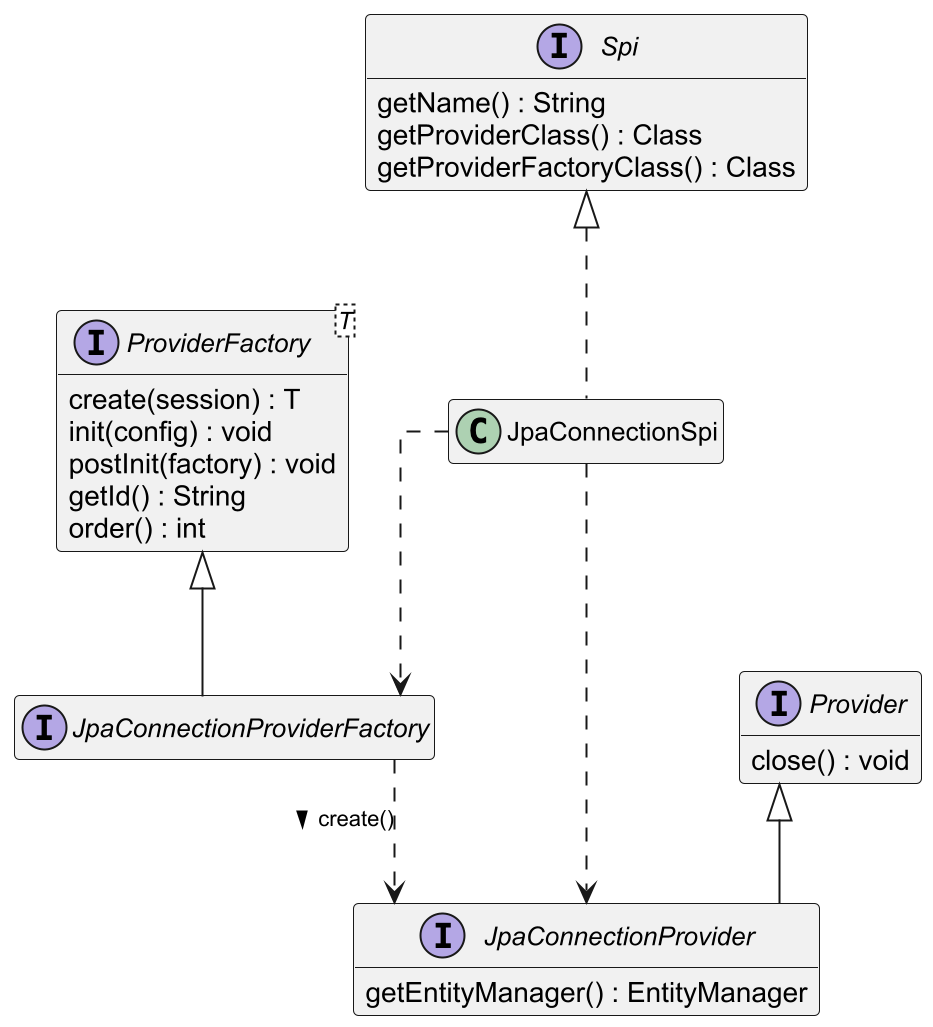
\includegraphics[width=0.7\textwidth]{images/spi-jpa-example-diagram.png}
    \caption{Пример реализации SPI: JPA-подключение в Keycloak}
    \label{fig:spi-jpa-example}
\end{figure}

Вся бизнес-логика реализуется не в наследниках интерфейса \texttt{Provider}. Например,
\texttt{JpaRealmProvider} реализует сразу несколько интерфейсов --- \texttt{RealmProvider}, 
\texttt{ClientProvider}, \texttt{GroupProvider}, \texttt{RoleProvider} --- и реализует всю работу с 
соответствующими сущностями на уровне базы данных через JPA. Каждый метод такого провайдера
выполняет конкретную операцию: создание, поиск, обновление или удаление объектов в 
рамках текущей сессии и транзакции.

\subsubsection*{Выбор провайдера по приоритету}

Алгоритм выбора следующий:

\begin{enumerate}
    \item Если явно задан провайдер через конфигурацию, то используется он; 
    \item Если зарегистрирована только одна фабрика, то используется она;
    \item Если зарегистрировано несколько фабрик, то выбирается та, у которой наибольшее значение \texttt{order()} среди всех с \texttt{order() > 0}. 
    \item Иначе используется фабрика с идентификатором default. 
\end{enumerate}


\subsection{Ключевые SPI и ProviderFactory для работы с базой данных}

\begin{itemize}
    \item \texttt{JpaConnectionProviderFactory} --- управляет созданием соединений с базой данных и жизненным циклом JPA \texttt{EntityManagerFactory};
    \item \texttt{LiquibaseConnectionProviderFactory} --- управляет подключением Liquibase для выполнения миграций;
    \item \texttt{DBLockProviderFactory} --- реализует распределённую блокировку для синхронизации при параллельном старте нескольких инстанций Keycloak;
    \item \texttt{RealmProviderFactory}, \texttt{ClientProviderFactory}, \texttt{ClientScopeProviderFactory} и прочие --- фабрики провайдеров для работы с основными сущностями данных.
\end{itemize}

\subsection{Механизм миграций и DBLockProvider.}
При старте Keycloak фабрика \texttt{JpaConnectionProviderFactory} инициирует создание схемы базы данных и
выполнение миграций через Liquibase. Поскольку Keycloak может запускаться в виде нескольких параллельных
узлов, необходима синхронизация: только один узел должен выполнять миграции в каждый момент времени.
Эту роль выполняет \texttt{DBLockProvider} --- провайдер глобальной распределённой блокировки, хранящий
состояние в отдельной таблице базы данных.

Блокировки разделены по пространству имён (\textit{namespace}):
\begin{itemize}
    \item \texttt{DATABASE} --- захватывается перед применением Liquibase-миграций (создание и обновление схемы таблиц);
    \item \texttt{KEYCLOAK\_BOOT} --- захватывается после завершения DDL-миграций для выполнения миграций данных (модельных миграций Keycloak).
\end{itemize}
Каждый узел ожидает снятия блокировки (по умолчанию до 900 секунд), после чего продолжает загрузку.

\subsection{Модель данных Keycloak}

Keycloak хранит данные в реляционных таблицах, отображаемых через Hibernate-аннотации на JPA-сущности.

Основные сущности Keycloak:

\begin{itemize}
    \item \textbf{Realm} --- область, содержащая конфигурацию, пользователей, клиентов, роли и группы; 
    \item \textbf{Client} --- OAuth/OIDC-клиент, зарегистрированный в realm; 
    \item \textbf{ClientScope} --- область видимости, определяющая набор claims в токене; 
    \item \textbf{Role} --- роль, назначаемая пользователям или клиентам; 
    \item \textbf{Group} --- группа пользователей с наследуемыми ролями; 
    \item \textbf{UserEntity} --- пользователь с атрибутами, учётными данными и привязкой к внешним провайдерам идентификации;
\end{itemize}

Cхема Keycloak включает более 80 таблиц и активно использует внешние ключи для обеспечения ссылочной целостности. 
Это является принципиальным ограничением при переносе на YDB.

\section{СУБД YDB}
В данном разделе рассмотрены технические особенности YDB, непосредственно
влияющие на проектирование интеграции с Keycloak.

\subsection{Ключевые свойства YDB}

\textbf{Масштабируемость.}
YDB поддерживает горизонтальное масштабирование: при росте нагрузки система может
автоматически перераспределять данные между узлами кластера без человеческого вмешательства.

\textbf{Транзакционная модель.}
В отличие от большинства распределённых СУБД, жертвующих транзакционными
гарантиями ради масштабируемости, YDB поддерживает полноценные ACID-транзакции
на нескольких узлах кластера. YDB поддерживает сериализуемую изоляцию транзакций и использует
\textit{оптимистичную блокировку}: конфликты не предотвращаются превентивно, а обнаруживаются
в момент коммита. Если за время выполнения транзакции другая транзакция успела изменить
затронутые строки, сервер откатывает её и возвращает ошибку \texttt{Transaction lock invalidated}.

YDB классифицирует ошибки на два типа. \textit{Non-retryable}-ошибки указывают на логические
нарушения (например, превышение схемных ограничений), и повтор бессмысленен.
\textit{Retryable}-ошибки носят временный характер: конфликт устранится сам собой, если
приложение повторит транзакцию с нуля. Ошибка \texttt{Transaction lock invalidated} относится
ко второму типу, однако повторяемая операция должна быть \textit{идемпотентной} ---
повторный вызов не должен приводить к дублированию эффектов.

\textbf{Отсутствие поддержки FOR UPDATE.} YDB не реализует пессимистичные блокировки строк.
Запросы с \texttt{SELECT ... FOR UPDATE} или \texttt{SELECT ... FOR SHARE} являются синтаксически некорректными в YQL.

\textbf{Обязательный первичный ключ.} Каждая таблица в YDB обязана иметь явно определённый первичный ключ.
Таблицы без первичного ключа создать невозможно.

\textbf{Отсутствие внешних ключей.} YDB не поддерживает декларативные ограничения внешних ключей.
Ссылочная целостность должна обеспечиваться на уровне приложения.

\textbf{Диалект YQL.} YDB использует YQL (Yandex Query Language) --- диалект SQL с рядом ограничений:

\begin{itemize}
    \item не поддерживаются ссылки на столбцы по порядковому номеру (\texttt{ORDER BY 1});
    \item не поддерживается \texttt{CONCAT()}, вместо них используется оператор \texttt{||};
    \item не поддерживаются операции \texttt{lower} и \texttt{upper}, вместо них используются \texttt{Unicode::ToLower} и \texttt{Unicode::ToUpper}
    \item каждый предикат в \texttt{JOIN ON} обязан ссылаться на столбцы
    \textit{обеих} сторон соединения --- условия фильтрации по одной таблице
    (вида \texttt{col = :param}) допускаются только в \texttt{WHERE};
    \item неявные декартовы произведения (перечисление таблиц через запятую в \texttt{FROM}) не поддерживаются ---
    вместо них требуется явный \texttt{CROSS JOIN}.
\end{itemize}

\subsection{Диалект Hibernate для YDB}

Hibernate --- это популярный ORM-фреймворк на Java, который абстрагирует работу с базой данных от 
конкретного SQL-диалекта.Для взаимодействия с конкретной СУБД Hibernate использует \textit{диалект} ---
класс, производный от \texttt{org.hibernate.dialect.Dialect}.
Диалект отвечает за отображение Java-типов на SQL-типы конкретной СУБД
и генерацию корректных SQL-выражений в её синтаксисе.

Для YDB существует реализация диалекта только для Hibernate 6, однако она содержит
ряд неточностей в обработке YQL-специфичных конструкций.
Поддержки Hibernate 7, используемого в Keycloak 26, не существовало.

\section{Аналоги и существующие решения}

На сегодняшний день существует реализация альтернативного хранилища для Keycloak на базе
Apache Cassandra --- проект \texttt{keycloak-cassandra-extension}.

Проект реализует замену стандартного JPA-хранилища на Apache Cassandra --- распределённую
NoSQL СУБД. Интеграция выполнена через механизм SPI Keycloak: расширение предоставляет
собственные реализации \texttt{DatastoreProvider} и отдельных провайдеров для каждого типа
сущностей (\texttt{UserProvider}, \texttt{RealmProvider}, \texttt{ClientProvider} и других).
Для работы с базой данных используется напрямую DataStax Java Driver, без Hibernate и JPA.

Ключевым отличием является то, что Cassandra не поддерживает реляционные транзакции.
Для обеспечения согласованности при конкурентных обновлениях используются
\textit{легковесные транзакции} (Lightweight Transactions, LWT).
Каждая сущность хранит поле \texttt{version},
и обновление выполняется только при совпадении версии: если другой процесс успел изменить
запись, операция отклоняется, и клиент должен повторить её.

Отсутствие реляционной модели потребовало полного переосмысления схемы данных. Если в
стандартном Keycloak каждое поле сущности соответствует отдельной колонке таблицы
(например, \texttt{JpaRealmEntity} содержит десятки типизированных колонок), то в
\texttt{keycloak-cassandra-extension} большинство свойств сущностей хранится в обобщённых
коллекциях --- ассоциативных массивах атрибутов (\texttt{map<text, list<text>>}).
Это позволяет не менять схему при добавлении новых полей, но лишает возможности использовать
SQL-поиск по конкретным полям. Для поддержки поиска пользователей создаются отдельные
индексные таблицы по выбранным атрибутам; поиск по произвольным атрибутам требует полного
обхода базы данных.

Проект поддерживает основные функции Keycloak, однако не реализует Authorization Services
и организации (Organizations). Миграции схемы выполняются через библиотеку Cassandra
Migration.

Таким образом, \texttt{keycloak-cassandra-extension} подтверждает принципиальную
возможность замены реляционного хранилища в Keycloak через механизм SPI, однако
потребовал полной переработки модели данных. Интеграция с YDB принципиально отличается:
YDB является реляционной СУБД с JDBC-драйвером и поддержкой Hibernate, что позволяет
сохранить существующую схему данных Keycloak. Основной задачей становится адаптация
Hibernate-диалекта к YQL и обработка retryable-ошибок транзакций YDB.

\chapterconclusion

В ходе анализа предметной области установлено, что Keycloak предоставляет механизм SPI,
позволяющий заменить стандартные JPA и Liquibase-провайдеры пользовательскими реализациями.
YDB поддерживает JDBC и Hibernate, что делает возможным сохранение существующей схемы данных
Keycloak при интеграции. Существующие решения для нереляционных СУБД требовали полной
переработки модели данных, тогда как подход с YDB позволяет ограничиться адаптацией
диалекта и обработкой специфичных для YDB ошибок транзакций.

\chapter{Проектирование решения}

\section{Общая архитектура модуля}

Модуль \texttt{keycloak-ydb-extension} встраивается в Keycloak через механизм SPI и состоит из трёх
подмодулей Maven:
\begin{itemize}
    \item \texttt{core/} --- основная реализация расширения на Kotlin, упакованная как shaded JAR
    и размещаемая в директории \texttt{providers/} Keycloak;
    \item \texttt{retry-proxy/} --- HTTP-прокси на Ktor, перехватывающий ответы с кодом 503
    и повторяющий запрос при временных ошибках YDB;
    \item \texttt{test/} --- интеграционные тесты с тестовым контейнером YDB.
\end{itemize}
Точкой входа служат файлы регистрации провайдеров в \texttt{META-INF/services/},
переопределяющие стандартные JPA- и Liquibase-провайдеры Keycloak.

\begin{figure}[H]
    \centering
    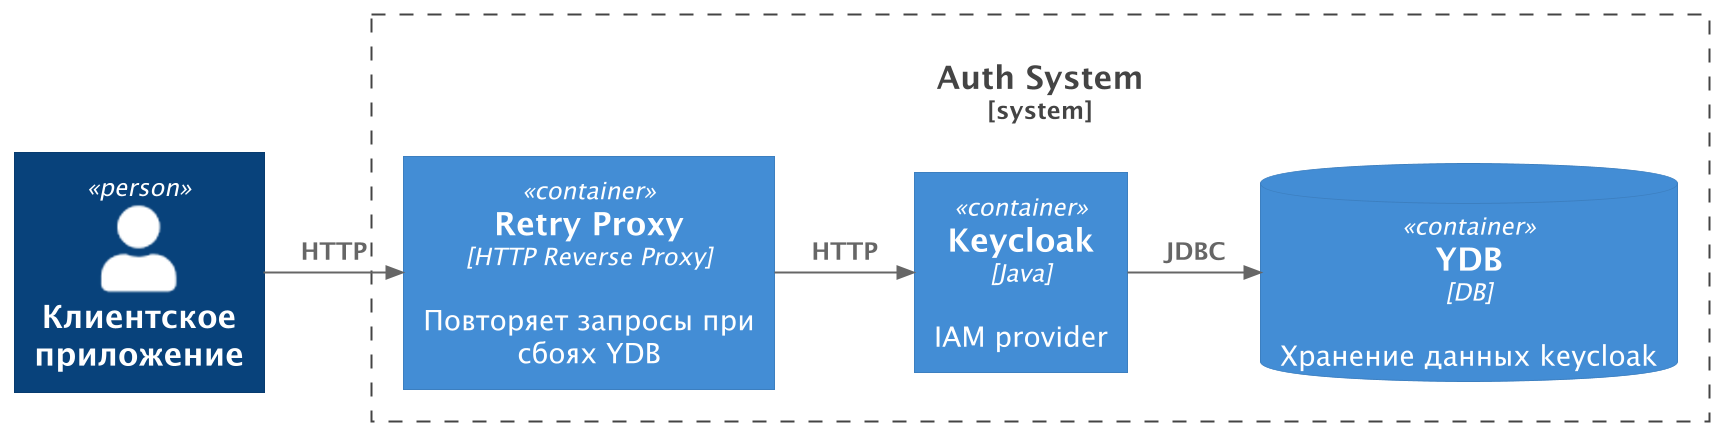
\includegraphics[width=\textwidth]{images/architecture-container-diagram.png}
    \caption{Контейнерная диаграмма системы}
    \label{fig:architecture-container}
\end{figure}

\begin{figure}[H]
    \centering
    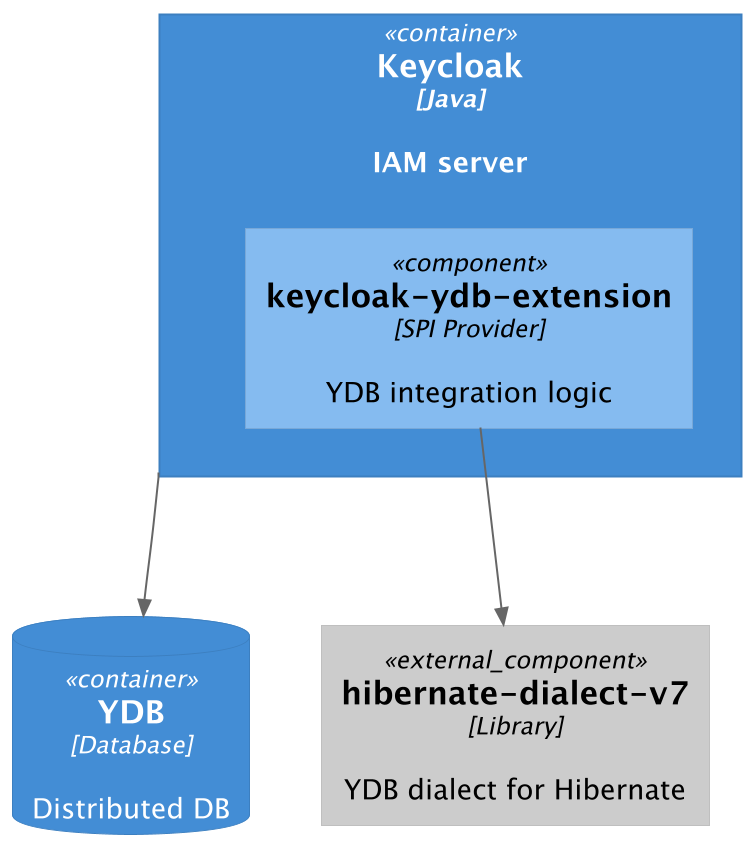
\includegraphics[width=0.5\textwidth]{images/keycloak-component-diagram.png}
    \caption{Компонентная диаграмма модуля keycloak-ydb-extension}
    \label{fig:keycloak-component}
\end{figure}

\section{Принципы проектирования схемы данных}

\subsection{Управление соединением с YDB}

Класс \texttt{YdbConnectionProviderFactoryImpl} является центральной точкой для
обеспечения связи Keycloak с YDB. Он реализует интерфейс 
\texttt{JpaConnectionProviderFactory} и в отличие от стандартного
провайдера Keycloak, который получает \texttt{EntityManagerFactory} через
механизмы Quarkus с пулом соединений Agroal, данная реализация самостоятельно
управляет пулом через HikariCP. Использование HikariCP обусловлено тем, 
что без явного пула соединений встроенный пул Hibernate быстро 
исчерпывается под нагрузкой и начинает возвращать ошибки. Agroal же 
недоступен вне контекста Quarkus. \texttt{EntityManagerFactory} создаётся с явно заданным
диалектом и драйвером YDB. В методе \texttt{postInit()} выполняется применение миграций схемы
с использованием распределённой блокировки \texttt{DBLockProvider}.
Транзакции оборачиваются в \texttt{YdbJpaKeycloakTransaction}, который
перехватывает retryable-ошибки YDB и преобразует их в HTTP 503.

\subsection{Анализ подходов к миграции схемы}

На начальном этапе были рассмотрены два подхода к созданию схемы базы данных.

\textbf{Подход 1: стандартные Liquibase-миграции Keycloak.}
Keycloak хранит историю изменений схемы в виде наборов миграций Liquibase, накопленных
за всю историю проекта (с версии 1.0). Набор включает более 70 XML-файлов, часть из
которых содержит ветвление по типу СУБД (\texttt{dbms="postgresql"}, \texttt{dbms="mssql"},
\texttt{dbms="oracle"} и т.\,д.) и условные сценарии миграции с \texttt{onFail="MARK\_RAN"}.
YDB в этом списке не предусмотрен, поэтому при попытке применить стандартные миграции
Liquibase выдаёт ошибки валидации. Миграции рассчитаны исключительно на поддерживаемые
СУБД и активно используют конструкции, которые YDB не поддерживает:
\begin{itemize}
    \item таблицы без явного первичного ключа (например, \texttt{SCOPE\_MAPPING}, \texttt{REDIRECT\_URIS});
    \item добавление первичного ключа отдельной командой после \texttt{CREATE TABLE};
    \item отсутствие \texttt{FOREIGN KEY};
    \item ограничения \texttt{UNIQUE CONSTRAINT} --- вместо них YDB поддерживает индексы \texttt{GLOBAL UNIQUE};
    \item добавление \texttt{NOT NULL} на существующую колонку через \texttt{ALTER TABLE} --- \texttt{NOT NULL} поддерживается только при создании таблицы;
    \item добавление значения по умолчанию на существующую колонку через отдельную операцию \texttt{addDefaultValue} --- YDB поддерживает \texttt{DEFAULT} только при создании таблицы;
    \item операция \texttt{RENAME COLUMN}.
\end{itemize}

\textbf{Подход 2: автоматическая генерация схемы через Hibernate (\texttt{HBM2DDL\_AUTO=update}).}
Hibernate умеет генерировать DDL напрямую из аннотаций JPA-сущностей.
Этот подход позволил создать некоторые таблицы, однако миграция не завершается успешно
из-за того, что в таблицах не было первичиных ключей

\textbf{Принятое решение: собственные Liquibase-миграции.}
Оба автоматических подхода оказались неприменимы без существенной доработки.
Принято решение написать собственный набор миграций,
воспроизводящих схему Keycloak с учётом ограничений YDB.
За основу взята финальная схема PostgreSQL, полученная после применения
всей истории стандартных Liquibase-миграций Keycloak.

При переносе схемы были применены следующие адаптации:
\begin{itemize}
    \item \textbf{Составные первичные ключи.}
    Связующие таблицы, не имеющие суррогатного ключа в PostgreSQL-схеме
    (например, \texttt{SCOPE\_MAPPING}, \texttt{REDIRECT\_URIS}, \texttt{USER\_ROLE\_MAPPING}),
    получили составной первичный ключ из колонок, образующих естественный идентификатор строки.

    \item \textbf{Замена \texttt{UNIQUE}-ограничений на \texttt{GLOBAL UNIQUE}-индексы.}
    Все уникальные ограничения PostgreSQL заменены индексами вида
    \texttt{GLOBAL UNIQUE}, обеспечивающими ту же семантику уникальности в YDB.

    \item \textbf{Удаление \texttt{FOREIGN KEY}-ограничений.}
    Объявления внешних ключей удалены; ссылочная целостность обеспечивается
    на уровне приложения. Для сохранения производительности поисковых запросов
    на колонках, бывших внешними ключами, созданы обычные \texttt{GLOBAL}-индексы.
\end{itemize}

\section{Разработка диалекта Hibernate для YDB}

На начальном этапе предполагалось использовать существующий \texttt{hibernate-dialect-v6},
поскольку в зависимостях Keycloak явно упоминался Hibernate 6.
Анализ зависимостей показал, что Keycloak 26 построен на Quarkus,
который транзитивно подтягивает Hibernate 7. Исправления, внесённые в
\texttt{hibernate-dialect-v6}, затрагивали API, несовместимый с Hibernate 7,
и не применялись. Таким образом, для корректной работы с Keycloak 26 потребовалось
создать отдельный модуль \texttt{hibernate-dialect-v7}.

Для обхода ограничения \texttt{FOR UPDATE} рассматривались два варианта:
переопределение конкретных методов провайдеров и добавление в диалект
настройки глобального игнорирования пессимистичных блокировок. Второй вариант принят как
менее трудоёмкий и не требующий изменений в коде провайдеров Keycloak.

\section{Архитектура механизма повторного выполнения транзакций}

При конкурентном доступе YDB может вернуть retryable-ошибку
(например \texttt{ABORTED} или \texttt{OVERLOADED}), означающую, что транзакцию
необходимо повторить с нуля.
Для её обработки разработана следующая архитектура: Keycloak при возникновении
такой ошибки возвращает клиенту HTTP 503 с маркером \texttt{ydb\_retryable}
в теле ответа. Вместо прямых обращений к Keycloak клиенты направляют запросы к
\texttt{retry-proxy} --- HTTP-прокси, который проксирует их в Keycloak
и при временном сбок YDB повторяет запрос автоматически, не возвращая ошибку клиенту.

Прокси отслеживает признак повторяемости по двум условиям одновременно:
код ответа равен 503 и тело содержит строку \texttt{ydb\_retryable}.
Все остальные ответы передаются клиенту без изменений.

Между повторными попытками прокси выдерживает задержку
по стратегии экспоненциального backoff, чтобы снизить нагрузку на сервер при пиковых конфликтах транзакций.

\chapterconclusion

В ходе проектирования определена трёхкомпонентная архитектура модуля: \texttt{core}
с SPI-провайдерами, \texttt{retry-proxy} для прозрачной обработки временных сбоев YDB
и \texttt{test} с интеграционными тестами. Для поддержки Hibernate 7 разработан отдельный
диалект \texttt{hibernate-dialect-v7}. Механизм повторного выполнения транзакций реализован
на уровне HTTP-прокси, что не требует изменений в клиентском коде и обеспечивает прозрачную
обработку retryable-ошибок.

\chapter{Реализация}

\section{Диалект Hibernate v7 для YDB}

Модуль \texttt{hibernate-dialect-v7} реализует класс \texttt{YdbDialect},
расширяющий базовый диалект Hibernate 7 для работы с YDB.
В ходе интеграции с Keycloak были выявлены и устранены следующие несовместимости.

\paragraph{Обработка OFFSET без LIMIT.}
Документация YDB описывает, что в случае когда в запросе присутствует
\texttt{OFFSET}, то \texttt{LIMIT} не обязателен.
На практике же запрос с \texttt{OFFSET} без \texttt{LIMIT} завершается ошибкой.
Keycloak в ряде запросов указывает только \texttt{OFFSET}, что приводило к сбою при выполнении.
В \texttt{YdbSqlAstTranslator} добавлена логика подстановки \texttt{LIMIT Long.MAX\_VALUE}
при наличии \texttt{OFFSET} без \texttt{LIMIT}.

\paragraph{Порядковые ссылки в ORDER BY.}
YDB не поддерживает конструкции вида \texttt{ORDER BY 1} (ссылка на столбец по порядковому
номеру). В диалекте переопределён метод \texttt{supportsOrdinalSelectItemReference()},
что вынуждает Hibernate генерировать явные имена столбцов.

\paragraph{Строковые функции.}
YDB не поддерживает стандартные функции \texttt{lower()}, \texttt{upper()} и
\texttt{concat()}. В диалекте они переопределены: \texttt{lower}/\texttt{upper}
транслируются в \texttt{Unicode::ToLower}/\texttt{Unicode::ToUpper},
\texttt{concat} --- в оператор \texttt{||}.

\paragraph{Игнорирование FOR UPDATE.}
Добавлена настройка \texttt{hibernate.dialect.ydb.ignore\_lock\_hints}.
При значении \texttt{true} методы генерации SQL возвращают запрос без
\texttt{FOR UPDATE}, что позволяет использовать Keycloak без переопределения
провайдеров, вызывающих запросы с пессимистичными блокировками.

% TODO: проверить влияние отсутствия пессимистичных блокировок на атомарность операций

\section{Реализация провайдеров Keycloak}

\subsection{YdbConnectionProviderFactoryImpl}

Центральным компонентом расширения является \texttt{Ydb\-Connection\-Provider\-Factory\-Impl},
реализующий интерфейс \texttt{JpaConnectionProviderFactory}.
Именно через этот интерфейс Keycloak получает доступ к хранилищу данных.
В методе \texttt{postInit()} выполняется запуск Liquibase-миграций и создание
\texttt{EntityManagerFactory} с YDB-диалектом.
При создании каждого провайдера \texttt{EntityManager} оборачивается двумя прокси:
стандартным прокси Keycloak и \texttt{YdbEntityManagerProxy}, который перехватывает
retryable-ошибки YDB и возвращает HTTP~503 для повторного выполнения запроса.
В качестве пула соединений используется HikariCP: встроенный пул Hibernate
при исчерпании соединений немедленно выбрасывает исключение, тогда как HikariCP
помещает запросы в очередь и ожидает освобождения соединения.

\subsection{Обработка транзакций}

Для корректной обработки ошибок YDB при фиксации транзакций реализован
\texttt{YdbJpaKeycloakTransaction}, перехватывающий исключения при коммите
и классифицирующий их как retryable с помощью утилиты \texttt{YdbErrorUtils}.
При обнаружении retryable-ошибки клиенту возвращается HTTP~503,
сигнализируя о необходимости повторного выполнения запроса.

\subsection{Переопределение провайдеров сущностей}

Поскольку YDB не поддерживает пессимистичные блокировки (\texttt{FOR UPDATE}),
на начальном этапе был реализован \texttt{YdbRealmProvider}, наследующий
\texttt{JpaRealmProvider}, с ручным каскадным удалением сущностей в методах
\texttt{removeRealm()}, \texttt{removeClient()} и \texttt{removeClientScope()}.
Однако в дальнейшем было принято решение игнорировать \texttt{FOR UPDATE}
непосредственно в Hibernate-диалекте, что позволило отказаться от переопределения
отдельных методов и упростить реализацию.

\subsection{Распределённые блокировки (YdbDBLockProvider)}

Стандартный \texttt{DBLockProvider} в Keycloak захватывает блокировку через
\texttt{SELECT FOR UPDATE}, что недоступно в YDB.
В рамках данной работы реализован \texttt{YdbDBLockProvider}, который захватывает
блокировку путём прямой записи в таблицу \texttt{DATABASECHANGELOGLOCK}:
при вызове \texttt{waitForLock(namespace)} в таблицу записывается информация
о захваченном пространстве имён, после чего другие вызовы \texttt{waitForLock}
с тем же пространством имён не могут получить блокировку.

Keycloak разделяет блокировки по пространствам имён: \texttt{DATABASE} для миграций
схемы и \texttt{KEYCLOAK\_BOOT} для инициализации модели данных.
Каждое пространство имён соответствует отдельной строке в таблице блокировок,
что позволяет узлам кластера независимо управлять разными фазами запуска.

Для генерации корректного SQL под YDB реализованы кастомные компоненты
на основе интерфейсов Liquibase: \texttt{YdbLockStatement}~--- описание операции
захвата блокировки, и \texttt{YdbLockSqlGenerator}~--- генератор SQL-запроса,
обновляющего строку таблицы блокировок для указанного пространства имён.

\section{Управление схемой данных через Liquibase}

Для управления схемой базы данных реализован \texttt{YdbLiquibaseConnectionProvider},
наследующий \texttt{DefaultLiquibaseConnectionProvider}.
Он переопределяет путь к файлу миграций: вместо стандартного changelog Keycloak
используется \texttt{ydb/db.changelog-master.xml}, а в качестве адаптера базы данных
применяется \texttt{YdbDatabase}~--- кастомная реализация интерфейса Liquibase для YDB.

Схема базы данных адаптирована с учётом ограничений YDB:
ограничения \texttt{UNIQUE CONSTRAINT} заменены на \texttt{GLOBAL UNIQUE INDEX},
внешние ключи (\texttt{FOREIGN KEY}) и ограничения \texttt{NOT NULL} через
\texttt{ALTER TABLE} исключены, поскольку YDB не поддерживает их добавление
после создания таблицы.
Значения по умолчанию задаются только при создании таблицы в \texttt{CREATE TABLE}.

Дополнительно настроен порог создания индексов (\texttt{indexCreationThreshold}),
по умолчанию равный 300\,000 строк~--- параметр оптимизации для работы с YDB
при больших объёмах данных.

\section{Переопределение именованных запросов}

Ряд стандартных JPQL-запросов Keycloak содержит синтаксические конструкции,
несовместимые с YQL. Выявлено два класса проблем.

Первый~--- неявный \texttt{CROSS JOIN} через \texttt{SELECT FROM A, B}:
Keycloak использует запросы, перечисляющие несколько сущностей через запятую
в \texttt{FROM} и связывающие их условием в \texttt{WHERE}, что YDB не поддерживает.
Такие запросы переписаны с явным \texttt{INNER JOIN}.

Второй~--- некорректные предикаты в \texttt{JOIN ON}: YDB требует,
чтобы каждое условие в \texttt{ON} ссылалось на столбцы обеих соединяемых таблиц.
Keycloak размещает в \texttt{ON} фильтры вида \texttt{column = :param},
что вызывает ошибку в YQL. Такие условия перенесены в \texttt{WHERE}.

Механизм переопределения использует стандартный механизм Keycloak:
файл \texttt{META-INF/queries-ydb.properties} содержит исправленные варианты
именованных JPQL-запросов. При старте метод \texttt{addSpecificNamedQueries()}
в \texttt{Ydb\-Connection\-Provider\-Factory\-Impl} загружает эти запросы
и регистрирует их в \texttt{EntityManagerFactory}, заменяя стандартные.

\chapterconclusion

В ходе реализации разработан диалект Hibernate 7 с устранёнными несовместимостями YQL,
реализованы SPI-провайдеры подключения к базе данных и управления схемой,
а также механизм переопределения именованных JPQL-запросов для обхода конструкций,
неподдерживаемых YDB. Совокупность реализованных компонентов обеспечивает работу
Keycloak с YDB в качестве основного хранилища данных.

\chapter{Тестирование}

\section{Интеграционное тестирование}

Для верификации корректности реализованных провайдеров разработан набор
интеграционных тестов.
Тесты запускаются против тестового контейнера YDB,
что исключает расхождение между поведением в тестах и в реальной среде.
Всего реализовано~47 тестовых случаев, охватывающих следующие области:

\begin{itemize}
    \item операции с областями (\texttt{RealmModelTest});
    \item управление клиентами и областями клиентов (\texttt{ClientModelTest},
          \texttt{ClientScopeModelTest}, \texttt{ClientScopeStorageTest});
    \item управление ролями и группами (\texttt{RoleModelTest}, \texttt{GroupModelTest});
    \item одноразовые объекты и временны́е смещения (\texttt{SingleUseObjectModelTest},
          \texttt{TimeOffsetTest});
    \item транзакционное поведение при retryable-ошибках (\texttt{StorageTransactionTest});
    \item события и аудит (\texttt{EventQueryTest}, \texttt{AdminEventQueryTest}).
\end{itemize}

\subsection{Тестирование распределённых блокировок}

Отдельное внимание уделено тестированию \texttt{YdbDBLockProvider}.
В классе \texttt{DBLockTest} проверяется корректность работы блокировок
при параллельном запуске нескольких потоков.
Тест \texttt{testLockConcurrentlyGeneral} запускает 20~потоков,
каждый из которых в~2~итерации захватывает и освобождает блокировку~---
семафор внутри теста гарантирует, что в каждый момент времени
критическую секцию проходит ровно один поток.
Тест \texttt{testTwoLocksCurrently} проверяет независимость блокировок
по разным пространствам имён: потоки с \texttt{DATABASE} и \texttt{KEYCLOAK\_BOOT}
могут работать одновременно, не блокируя друг друга.
Тест \texttt{testTwoNestedLocksCurrently} проверяет вложенные блокировки:
часть потоков захватывает два уровня блокировки последовательно,
остальные~--- только верхний уровень.

\section{Нагрузочное тестирование}

Для оценки производительности реализованного решения разработан стенд нагрузочного
тестирования на основе инструмента \texttt{keycloak-benchmark},
использующего Gatling в качестве движка генерации нагрузки.

Стенд поддерживает три конфигурации инфраструктуры:
\begin{itemize}
    \item Keycloak~+ локальный YDB (Docker) с retry-proxy;
    \item Keycloak~+ удалённый YDB с retry-proxy;
    \item Keycloak~+ PostgreSQL~--- для сравнительного анализа.
\end{itemize}

Перед запуском тестов скрипт \texttt{setup-test-realm.py} создаёт тестовые клиенты, роли, группы и пользователи.
Нагрузочный тест запускается командой:

\begin{verbatim}
./run.sh <scenario> <users-per-sec> [duration-sec]
\end{verbatim}

Для нагрузочного тестирования выбраны сценарии, покрывающие два ключевых
класса операций Keycloak.
Первый класс --- \textbf{аутентификация}: это наиболее часто выполняемые
операции в production-системе, поскольку каждое обращение клиентского
приложения к защищённому ресурсу инициирует хотя бы одно взаимодействие
с Keycloak.
Второй класс --- \textbf{управление пользователями}: операции создания,
поиска и удаления пользователей характеризуются интенсивной записью
в основные таблицы YDB и вторичные индексы, что делает их показательными
с точки зрения поведения базы данных под конкурентной нагрузкой.

В рамках данной работы протестированы следующие сценарии:

\begin{table}[H]
\centering
\begin{tabular}{|l|l|}
\hline
\textbf{Сценарий} & \textbf{Описание} \\
\hline
CreateUsers & Создание пользователя и получение списка пользователей \\
\hline
AuthorizationCode & Аутентификация по Authorization Code Flow \\
\hline
CreateDeleteUsers & Создание, получение списка и удаление пользователя \\
\hline
ClientSecret & Аутентификация по Client Credentials Flow \\
\hline
LoginUserPassword & Аутентификация через браузерную форму логина \\
\hline
\end{tabular}
\caption{Сценарии нагрузочного тестирования}
\end{table}

Результаты каждого прогона сохраняются в директорию \texttt{results/}
в виде HTML-отчётов Gatling с метриками пропускной способности (Запросов в секунду),
времени ответа (p50, p95, p99) и долей ошибок.

В рамках данной работы проведено предварительное нагрузочное тестирование
на локальной машине разработчика с YDB, запущенной в Docker-контейнере.
Тестирование на выделенном стенде с полноценным экземпляром YDB запланировано
как следующий этап работы.

Для сценария \texttt{CreateUsers} выполнено четыре прогона.
Сценарий включает три шага на итерацию: получение токена сервисного аккаунта,
создание пользователя и получение списка пользователей.
Прогоны 1 и 2 выполнены с синхронным индексом (\texttt{GLOBAL}),
прогоны 3 и 4~--- после оптимизации схемы (\texttt{GLOBAL ASYNC}).


\begin{table}[H]
\centering
\begin{tabular}{|l|c|c|c|c|c|c|}
\hline
\textbf{Прогон} & \textbf{Индекс} & \textbf{users/sec} & \textbf{Запросов} & \textbf{Ошибок} & \textbf{req/s} & \textbf{p50} \\
\hline
Прогон 1 & GLOBAL       & 30 & 5\,625  & 0\%     & 87  & 11 мс \\
Прогон 2 & GLOBAL       & 35 & 6\,250  & 5{,}1\% & 51  & 2\,818 мс \\
Прогон 3 & GLOBAL ASYNC & 35 & 6\,561  & 0\%     & 101 & 10 мс \\
Прогон 4 & GLOBAL ASYNC & 45 & 8\,436  & 0\%     & 128 & 15 мс \\
\hline
\end{tabular}
\caption{Результаты сценария CreateUsers}
\label{tab:load-create-users}
\end{table}

Первый прогон завершился успешно: все 5\,625~запросов выполнены без ошибок,
пропускная способность составила 87~запросов в секунду,
медианное время ответа~--- 11~мс, 99-й перцентиль~--- 21~мс.

Второй прогон при увеличении нагрузки до 35~пользователей в секунду показал
5{,}1\%~ошибок и резкую деградацию латентности: медианное время ответа выросло
до 2\,818~мс, 99-й перцентиль~--- до 59\,085~мс, часть запросов превысила
60-секундный таймаут Gatling.
Анализ логов Keycloak выявил конкретную причину~--- конфликты блокировок
на вторичном индексе таблицы пользователей:

\begin{verbatim}
Transaction locks invalidated.
Table: /local/USER_ENTITY/idx_user_service_account/indexImplTable
\end{verbatim}

При создании пользователей все параллельные транзакции одновременно
обновляют один и тот же физический файл вторичного индекса
\texttt{idx\_user\_service\_account}, что приводит к инвалидации блокировок YDB
(аналог \texttt{ABORTED}).
Реализованный retry-proxy выполнял до 10~повторных попыток с экспоненциальной
задержкой, поэтому овторные попытки увеличивали количество конкурирующих транзакций,
что дополнительно усиливало нагрузку и приводило к росту числа ошибок.
После исчерпания попыток proxy возвращал 502, которые Gatling фиксировал как
ошибки; наиболее долгие запросы (до 60~с) завершились таймаутом на стороне
Gatling в ожидании ответа proxy.

Для устранения проблемы индекс \texttt{idx\_user\_service\_account} был переведён
из синхронного режима (\texttt{GLOBAL}) в асинхронный (\texttt{GLOBAL ASYNC}).
В YDB синхронный индекс обновляется в рамках той же транзакции, что и основная
таблица: при параллельных вставках все потоки конкурируют за одни и те же
строки одного partition индекса по \texttt{REALM\_ID}, провоцируя лавину
конфликтов.
Асинхронный индекс обновляется отдельно от основной транзакции~---
конкуренция на файле индекса исчезает.
Для \texttt{idx\_user\_service\_account} подобная задержка допустима:
индекс используется исключительно для поиска сервисных аккаунтов,
а не в критичном пути аутентификации.

Третий прогон с \texttt{GLOBAL ASYNC} при той же нагрузке 35~пользователей
в секунду завершился без единой ошибки: 6\,561~запрос, медианное время~--- 10~мс,
99-й перцентиль~--- 61~мс, максимальное время~--- 3\,093~мс.
Логи Keycloak фиксировали единичные retryable-ошибки на основной таблице
\texttt{USER\_ENTITY}, которые retry-механизм
(\texttt{YdbJpaKeycloakTransaction}) разрешал прозрачно~---
без эскалации до ошибок на стороне клиента.
Максимальное время ответа 3\,093~мс соответствует одному полному циклу
повторной попытки с экспоненциальной задержкой.

Четвёртый прогон подтвердил устойчивость оптимизации при дальнейшем
увеличении нагрузки до 45~пользователей в секунду: 8\,436~запросов,
0~ошибок, медианное время~--- 15~мс, 99-й перцентиль~--- 283~мс.
Среднеквадратическое отклонение 143~мс при среднем 28~мс указывает на наличие
единичных длительных повторных попыток (максимум 5\,366~мс), однако все они
завершились успешно в рамках retry-бюджета.
Оба SLA~--- доля ошибок не более 0\% и среднее время ответа не более
300~мс~--- выполнены.

Для сценария \texttt{CreateUsers} также был проведён аналогичный прогон с использованием PostgreSQL.

\begin{table}[H]
\centering
\begin{tabular}{|l|c|c|c|c|c|c|}
\hline
\textbf{users/sec} & \textbf{Запросов} & \textbf{Ошибок} & \textbf{RPS} & \textbf{p50} & \textbf{p99} \\
\hline
190 & 37\,500 & 0\% & 577 & 1 мс & 4 мс \\
\hline
\end{tabular}
\caption{Результаты сценария CreateUsers (PostgreSQL)}
\label{tab:load-create-users-postgres}
\end{table}

Все 37,500 запросов выполнены успешно без ошибок.
Медианное время ответа составило 1~мс, 95-й перцентиль — 2~мс, 99-й перцентиль — 4~мс.
Максимальное время ответа не превысило 141~мс.

Полученные результаты демонстрируют, что PostgreSQL эффективно справляется со сценарием,
включающим операции записи, даже при высокой интенсивности нагрузки.
В отличие от YDB, где при аналогичных сценариях наблюдаются конфликты транзакций
и рост количества повторных попыток, PostgreSQL обеспечивает стабильную
латентность и отсутствие ошибок.

Следует отметить, что различие в результатах также связано с условиями проведения тестирования:
PostgreSQL и Keycloak запускались локально в оптимизированной конфигурации,
в то время как YDB использовалась в Docker-контейнере, что ограничивает доступные ресурсы
и влияет на поведение системы под нагрузкой.

Для сценария \texttt{AuthorizationCode} выполнено два прогона.
Сценарий моделирует полный цикл аутентификации пользователя по протоколу
Authorization Code Flow и включает четыре шага на итерацию:
открытие страницы входа, ввод логина и пароля, обмен кода авторизации
на токен и выход из системы.

\begin{table}[H]
\centering
\begin{tabular}{|l|c|c|c|c|c|c|}
\hline
\textbf{Прогон} & \textbf{users/sec} & \textbf{Запросов} & \textbf{Ошибок} & \textbf{req/s} & \textbf{p50} & \textbf{p99} \\
\hline
Прогон 1  & 90  & 22\,500 & 0\%  & 341  & 19 мс       & 93 мс \\
Прогон 2  & 100 & 25\,000 & 0\%  & 338  & 1\,686 мс   & 3\,811 мс \\
\hline
\end{tabular}
\caption{Результаты сценария AuthorizationCode}
\label{tab:load-auth-code}
\end{table}

Первый прогон при 90~пользователях в секунду завершился полностью успешно:
все 22\,500~запросов выполнены без ошибок, медианное время ответа составило
19~мс, 99-й перцентиль~--- 93~мс, максимальное время ответа~--- 355~мс.

Второй прогон при увеличении нагрузки до 100~пользователей в секунду
не дал ошибок, однако медианное время ответа выросло до 1\,686~мс,
99-й перцентиль~--- до 3\,811~мс, а 67\% запросов превысили 1\,200~мс.
Пропускная способность при этом осталась практически неизменной (338~ запросов в секунду),
что указывает на достижение точки насыщения: система успевает
обработать все запросы, но накапливает очередь.

Сценарий \texttt{AuthorizationCode} выдерживает значительно более высокую
нагрузку, чем \texttt{CreateUsers}, по двум причинам.
Во-первых, сценарий является преимущественно читальным: чтение конфигурации
области и клиента, поиск пользователя по имени~--- всё это операции чтения
без конкурентных изменений одних и тех же строк.
Во-вторых, единственные операции записи~--- создание сессии и токена~---
используют уникальные UUID-идентификаторы, что полностью исключает конфликты
транзакций в YDB и, как следствие, ошибки типа \texttt{ABORTED}.
В сценарии \texttt{CreateUsers} все потоки конкурентно пишут в одни и те же
таблицы пользователей, что при 40~пользователях в секунду уже приводит
к лавинообразному нарастанию retryable-ошибок YDB.

Для сравнения производительности был проведён аналогичный прогон сценария \texttt{AuthorizationCode} с использованием PostgreSQL.
\begin{table}[H]
\centering
\begin{tabular}{|l|c|c|c|c|c|c|}
\hline
\textbf{users/sec} & \textbf{Запросов} & \textbf{Ошибок} & \textbf{Запросов в секунду} & \textbf{p50} & \textbf{p99} \\
\hline
100 & 25,000 & 0\% & 379 & 7 мс & 22 мс \\
\hline
\end{tabular}
\caption{Результаты сценария AuthorizationCode (PostgreSQL)}
\label{tab:load-auth-code-postgres}
\end{table}

Все 25,000 запросов выполнены успешно без ошибок.
Медианное время ответа составило 7~мс, 95-й перцентиль — 16~мс, 99-й перцентиль — 22~мс.
Максимальное время ответа не превысило 354~мс.
Полученные результаты демонстрируют, что PostgreSQL обеспечивает более стабильные результаты
по тем же причинам что и при сценарии CreateUsers

Для сценария \texttt{ClientSecret} выполнено три прогона.
Сценарий моделирует Client Credentials Flow: один POST-запрос на эндпоинт
токена с \texttt{client\_id} и \texttt{client\_secret} без участия пользователя.
Это наиболее лёгкий сценарий~--- нет браузерного флоу, кук и редиректов.

\begin{table}[H]
\centering
\begin{tabular}{|l|c|c|c|c|c|c|}
\hline
\textbf{Прогон} & \textbf{users/sec} & \textbf{Запросов} & \textbf{Ошибок} & \textbf{Запросов в секунду} & \textbf{p50} & \textbf{p99} \\
\hline
Прогон 1  & 200 & 12\,500 & 0\%     & 192  & 7 мс   & 112 мс \\
Прогон 2  & 400 & 25\,000 & 0\%     & 385  & 7 мс   & 18 мс \\
Прогон 3  & 800 & 50\,000 & 42{,}8\% & 758  & ---    & --- \\
\hline
\end{tabular}
\caption{Результаты сценария ClientSecret}
\label{tab:load-client-secret}
\end{table}

Прогоны при 200 и 400~пользователях в секунду прошли без ошибок.
Примечательно, что при 400~req/s показатели оказались даже лучше, чем при 200:
медианное время~--- 7~мс, 99-й перцентиль~--- 18~мс, стандартное отклонение~---
7~мс. Это объясняется прогревом JVM и стабилизацией пула соединений HikariCP.

При увеличении нагрузки до 800~req/s возникли ошибки, однако их причина~---
не Keycloak и не YDB, а ограничение
локальной машины: при таком количестве запросов в секунду заканчиваются
свободные сетевые порты операционной системы, и Gatling не может открыть
новые соединения (\texttt{BindException: Can't assign requested address}).
Таким образом, реальный предел производительности сервера выше 400~req/s,
но точно измерить его на одной машине, где работают и клиент, и сервер,
не представляется возможным.

Для сценария \texttt{CreateDeleteUsers} выполнено четыре прогона при нагрузке
30 и~40~пользователей в секунду с~типами индекса \texttt{GLOBAL} и~\texttt{GLOBAL ASYNC}.
Сценарий моделирует полный жизненный цикл пользователя: получение токена
сервисного аккаунта, создание пользователя, получение списка пользователей
и удаление созданного пользователя~--- четыре запроса на одну итерацию.
Все прогоны выполнялись на базе данных, уже содержавшей данные пользователей,
накопленные в~предшествующих прогонах \texttt{CreateUsers}.

\begin{table}[H]
\centering
\begin{tabular}{|l|c|c|c|c|c|c|}
\hline
\textbf{Индекс} & \textbf{users/sec} & \textbf{Запросов} & \textbf{Ошибок} & \textbf{req/s} & \textbf{p50} & \textbf{p99} \\
\hline
GLOBAL ASYNC & 30 & 7\,500  & 0\%          & 114 & 10 мс  & 70 мс     \\
GLOBAL ASYNC & 40 & 9\,996  & $\approx$0\% & 151 & 13 мс  & 1\,432 мс \\
GLOBAL       & 30 & 6\,219  & 10{,}4\%     & 51  & \multicolumn{2}{c|}{деградация} \\
GLOBAL       & 40 & 7\,290  & 17{,}8\%     & 54  & \multicolumn{2}{c|}{деградация} \\
\hline
\end{tabular}
\caption{Результаты сценария CreateDeleteUsers}
\label{tab:load-create-delete-users}
\end{table}

С~\texttt{GLOBAL ASYNC} оба прогона завершились практически без ошибок:
p50~--- 10–13~мс, p99~--- 70~мс и~1\,432~мс соответственно.
С~\texttt{GLOBAL} на~той~же базе данных наблюдалась катастрофическая деградация:
ошибки~10\% и~18\%, количество запросов в секунду упал с~ожидаемых 114/151 до~51/54,
среднее время ответа~--- свыше~11~секунд,
часть запросов исчерпывала 60-секундный таймаут Gatling.

Причина~--- конкуренция операций при смешанной нагрузке.
Шаг <<Получение списка пользователей>> (\texttt{List Users})
при заполненной таблице удерживает широкие читающие блокировки (\texttt{S-locks}).
Параллельные \texttt{CREATE} и~\texttt{DELETE} запрашивают
эксклюзивные блокировки (\texttt{X-locks})~--- возникает конфликт,
YDB отвечает ошибкой \texttt{ABORTED}.
При \texttt{GLOBAL} каждая операция \texttt{CREATE} синхронно записывает
в~партицию индекса, что~создаёт дополнительное конкурентное давление,
которое retry-proxy уже не~успевает компенсировать, и~отказы
распространяются на~все типы запросов.
\texttt{GLOBAL ASYNC} убирает синхронную запись в~индекс из~критического пути,
снижая суммарное число конкурирующих транзакций~--- и~retry-механизм
справляется с~оставшимися конфликтами прозрачно.

Для сценария \texttt{LoginUserPassword} выполнено два прогона.
Сценарий моделирует аутентификацию через браузерную форму: открытие страницы логина
и отправка формы с именем пользователя и паролем~--- два HTTP-запроса на итерацию.
В отличие от \texttt{AuthorizationCode}, сценарий не выполняет обмен кода на токен
и не завершает сессию logout'ом.

\begin{table}[H]
\centering
\begin{tabular}{|l|c|c|c|c|c|c|}
\hline
\textbf{Прогон} & \textbf{users/sec} & \textbf{Запросов} & \textbf{Ошибок} & \textbf{Запросов в секундк} & \textbf{p50} & \textbf{p99} \\
\hline
Прогон 1  & 90  & 11\,250 & 0\%      & 170  & 29 мс  & 203 мс \\
Прогон 2  & 200 & 22\,744 & 19{,}1\% & 274  & ---    & --- \\
\hline
\end{tabular}
\caption{Результаты сценария LoginUserPassword}
\label{tab:load-login-password}
\end{table}

При 90~пользователях в секунду прогон завершился без ошибок: 11\,250~запросов,
среднее время ответа~--- 31~мс, 99-й перцентиль~--- 203~мс, все запросы уложились в 800~мс.

При увеличении нагрузки до 200~пользователей в секунду возникли ошибки (19{,}1\%).
Все ошибочные запросы вернули статус~502 и имели время ответа ровно 10~секунд
(стандартное отклонение~--- 9~мс)~--- это в точности значение \texttt{connectTimeout}
прокси-сервера.
При перегрузке Keycloak перестаёт принимать новые TCP-соединения;
прокси не может подключиться в течение 10~секунд и возвращает \texttt{502 Bad Gateway}
без логирования (исключение перехватывается без retry и без записи в лог).

Важно понимать природу этого ограничения.
В Keycloak онлайн-сессии не хранятся в базе данных~--- они живут в Infinispan кэше.
Keycloak предоставляет две реализации \texttt{UserSessionProviderFactory}:
\texttt{InfinispanUserSessionProviderFactory} (embedded-режим, Infinispan встроен
в процесс Keycloak) и \texttt{RemoteUserSessionProviderFactory} (внешний Infinispan-кластер).
Обе реализации основаны на Infinispan; замена этого слоя на произвольную реляционную
базу данных через SPI не предусмотрена.
В базу данных (через JPA и, следовательно, в YDB) пишутся только \textbf{offline-сессии}
через \texttt{UserSessionPersisterProvider}~--- эта часть в реализации присутствует
(таблицы \texttt{OFFLINE\_USER\_SESSION} и \texttt{OFFLINE\_CLIENT\_SESSION}).

Таким образом, деградация при 200~req/s~--- это ограничение JVM-кучи и Infinispan,
а не YDB.
Сценарий \texttt{LoginUserPassword} без logout'а накапливает сессии в памяти процесса:
200~req/s~$\times$~35~с~$\approx$~7\,000~объектов сессий в heap,
что приводит к давлению на GC и насыщению пула потоков Keycloak.
В реальном развёртывании сессии имеют TTL и периодически вытесняются Infinispan'ом,
поэтому подобная деградация не возникала бы при стабильной нагрузке.

Проведённое нагрузочное тестирование в условиях локальной разработки показало,
что ключевые сценарии Keycloak --- аутентификация и управление пользователями ---
функционируют корректно и демонстрируют приемлемую производительность.
Сценарии, основанные преимущественно на чтении, устойчиво выдерживают
сотни запросов в секунду; сценарии с интенсивной записью ограничены конкуренцией
транзакций YDB, которая эффективно снижается переходом на асинхронные вторичные
индексы.
Вместе с тем полученные результаты не отражают поведение системы в реальном
production-окружении, ведь тестирование проводилось на одной машине с YDB в
Docker-контейнере, что существенно ограничивает как ресурсы, так и масштаб нагрузки.
Тестирование на выделенном стенде с полноценным кластером YDB, соответствующим
production-конфигурации, запланировано как следующий шаг и позволит получить
окончательные выводы о производительности решения.

%% Макрос для заключения. Совместим со старым стилевиком.
\startconclusionpage

В рамках данной работы разработан программный модуль, обеспечивающий интеграцию
Keycloak с YDB в качестве основного хранилища данных.

Проведён анализ архитектуры Keycloak и особенностей YDB, определяющих требования
к адаптации: несовместимость ряда SQL-конструкций с диалектом YQL и необходимость
обработки временных сбоев при конкурентных транзакциях.
Реализован Hibernate-диалект, обеспечивающий корректную работу Keycloak с YDB,
и набор SPI-провайдеров, отвечающих за управление соединениями, выполнение миграций
схемы и распределённую блокировку при запуске.
Разработан retry-механизм на уровне JDBC, прозрачно перехватывающий временные сбои
транзакций YDB и повторяющий их без изменений в коде приложения.
Выполнено нагрузочное тестирование на ключевых сценариях Keycloak, подтверждающее
работоспособность решения и позволившее выявить направления дальнейшей оптимизации.

Разработанный модуль позволяет организациям, использующим YDB в своей инфраструктуре,
развернуть Keycloak без необходимости поддерживать отдельную реляционную СУБД.
Модуль опубликован в открытом доступе и является частью экосистемы YDB Java Dialects.

В качестве направлений дальнейшей работы планируется проведение нагрузочного
тестирования на выделенном production-стенде с полноценным кластером YDB
для получения объективных данных о производительности в реальных условиях эксплуатации.

\nocite{*}
\printmainbibliography

%% После этой команды chapter будет генерировать приложения, нумерованные русскими буквами.
%% \startappendices из старого стилевика будет делать то же самое
\appendix

\end{document}
